% vim: et sw=2 ts=2 sts=2

\section{Heurísticas para Solução do Problema}
\frame{
  \frametitle{Heurísticas para Solução do Problema}
  \begin{block}{}
    \begin{enumerate}
      \item Lógica Nebulosa
      \item \textit{Conditional Random Fields} (CRFs)
      \item \textit{Ant Colony Optimization} (ACO)
      \item \textit{Simulated Annealing} (SA)
      \item Algorítimo Genético (AG)
      \item Redes Neurais
    \end{enumerate}
  \end{block}
}

\frame{
  \frametitle{Lógica Nebulosa}
  \begin{block}{}
    \begin{figure}
      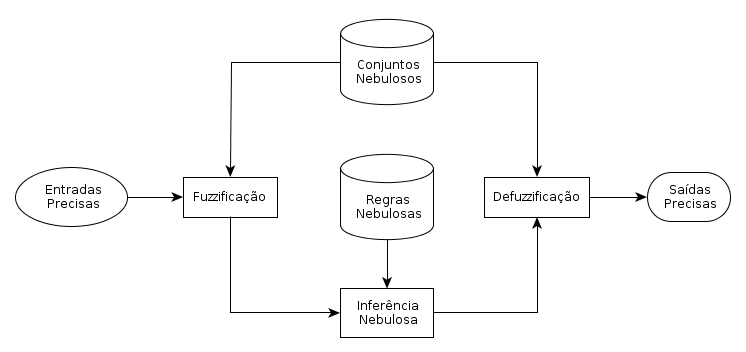
\includegraphics[width=0.8 \linewidth]
      {imgs/arquitetura_fuzzy}
      \caption{Arquitetura Funcional Genérica de um Sistema
      Nebuloso}
    \end{figure}
  \end{block}
}

\frame{
  \frametitle{Lógica Nebulosa}
  \begin{block}{}
    \textbf{Exemplo} Determinar o valor da apólice de seguro
    a ser paga pelo cliente João, cuja idade é 35 anos e a
    pressão arterial é de (130,75). As regras são:
    \begin{itemize}
      \item \emph{SE} idade é \textit{meia-idade} \emph{E}
            pressão arterial é \textit{baixa} \emph{ENTÃO}
            seguro é \textit{baixo}
      \item \emph{SE} é \textit{jovem} \emph{E} pressão
            arterial é \textit{alta} \emph{ENTÃO} seguro
            é \textit{alto}
    \end{itemize}
  \end{block}
}

%\frame{
%  \frametitle{Lógica Nebulosa}
%  \begin{block}{}
%    Se $\mu_{meia-idade}(35)= 0.8, \mu_{jovem}(35)= 0.6,
%    \mu_{Alta}(130,70)=0.5$ e $\mu_{Baixa}=0.6$, tem-se:
%    \begin{itemize}
%      \item $0.8$ \emph{E} $0.6$ = $Min \lbrace 0.8,
%      0.6\rbrace = 0.6 = \mu_{seguro-baixo}(X_1)$
%      \item $0.6$ \emph{E} $0.5$ = $Min \lbrace 0.6,
%      0.5\rbrace = 0.5 = \mu_{seguro-alto}(X_2)$
%    \end{itemize}
%  \end{block}
%  \begin{block}{}
%    Aplicando o processo de defuzzificação, obtem-se:
%    \begin{itemize}
%      \item $X_1 = 700$ e $X_2 = 800$
%    \end{itemize}
%	Assim, o valor final da apólice de seguro seria:
%	\[
%	Seguro = \frac{(0.6 \times 700)+(0.5 \times 800)}
%	{0.6+0.5} = 745.45 reais
%	\]
%  \end{block}
%}

\frame{
  \frametitle{Lógica Nebulosa}
  \begin{block}{}
    \begin{figure}
      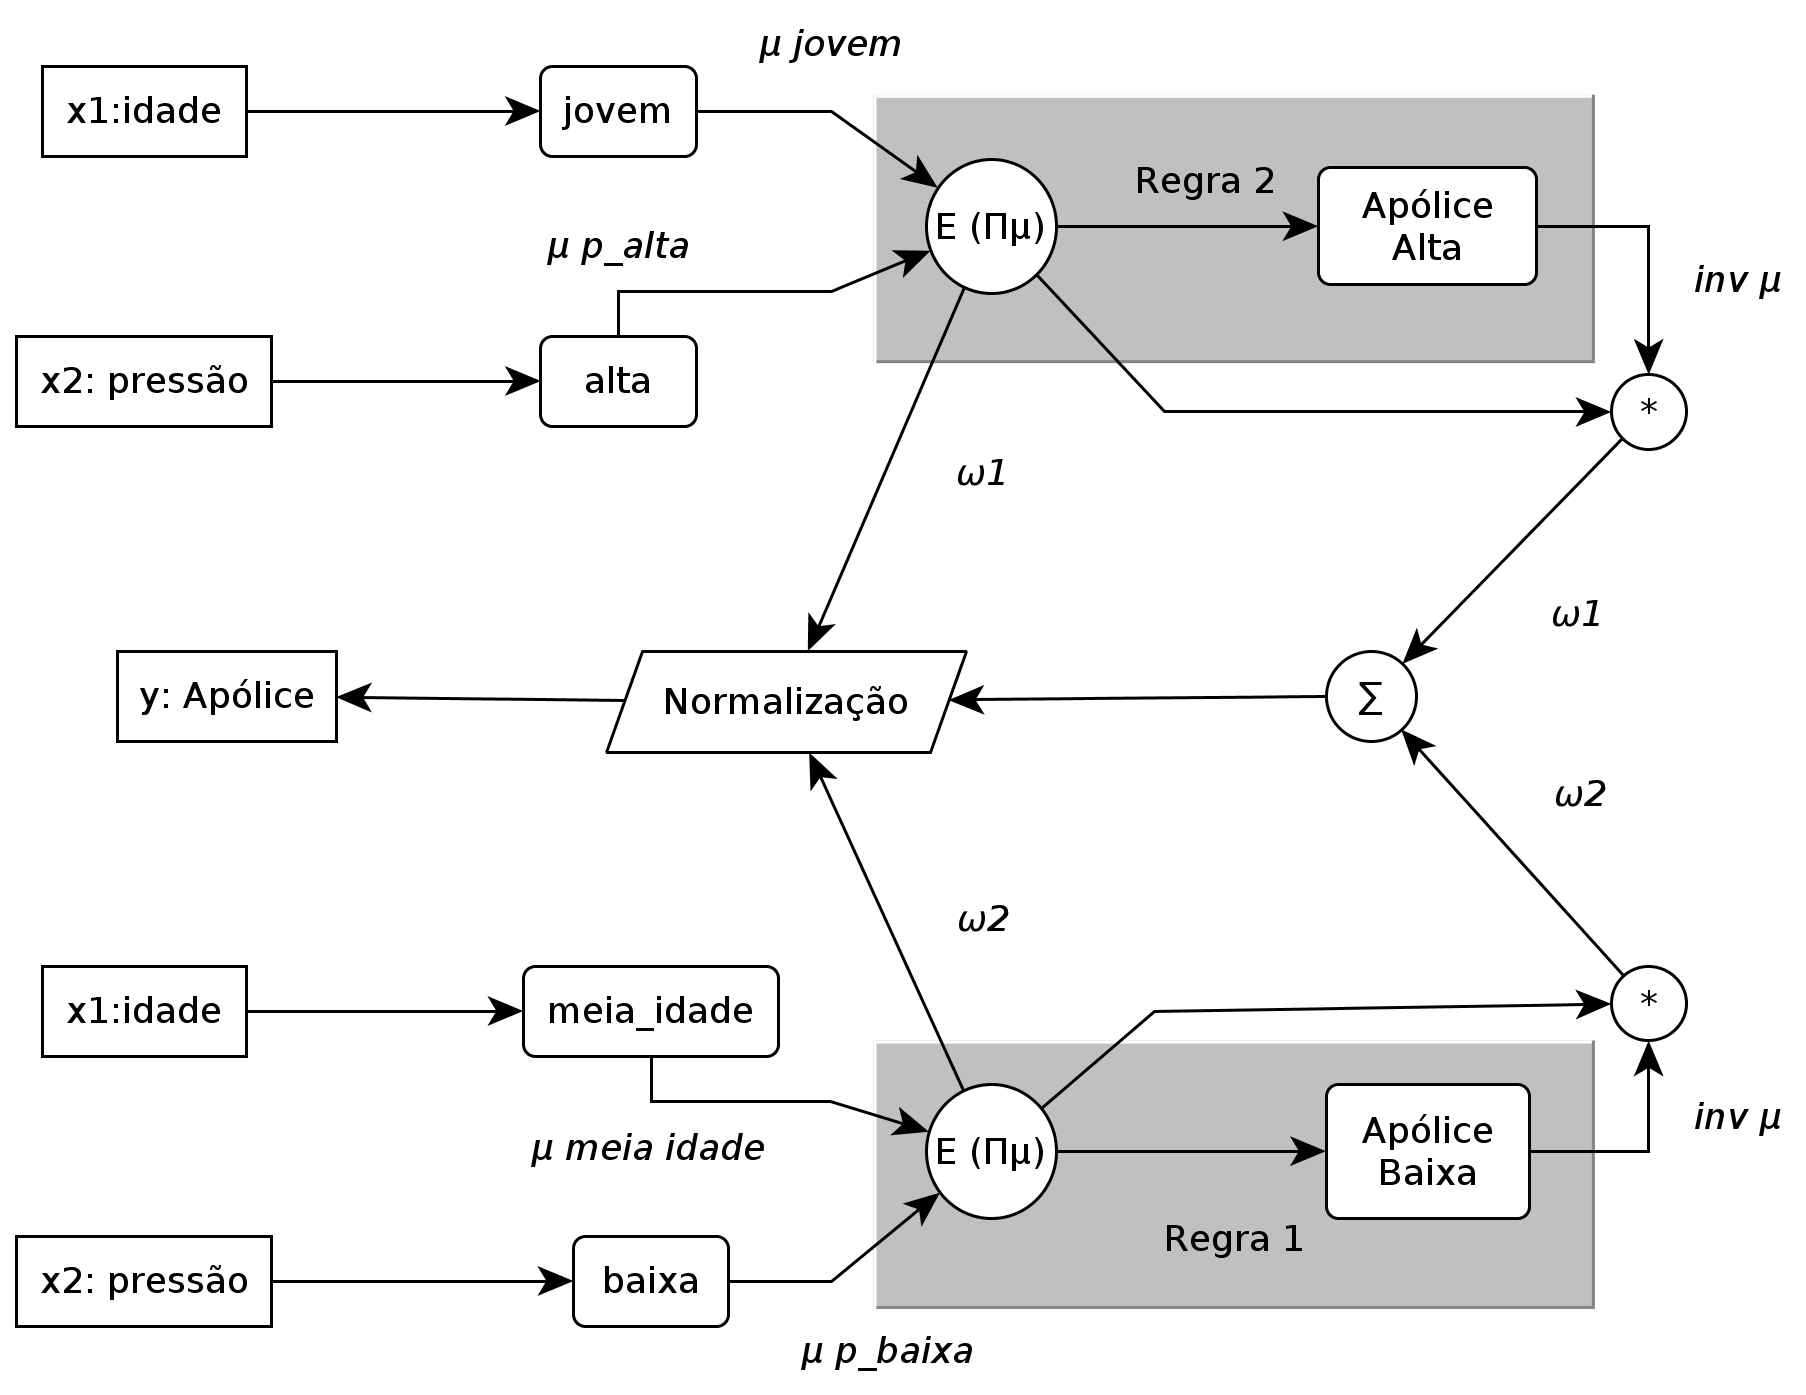
\includegraphics[width =0.6 \linewidth]
      {imgs/ex_logica_fuzzy}
      \caption{Exemplo de Aplicação}
    \end{figure}
  \end{block}
}

\frame{
  \frametitle{Lógica Nebulosa (SAM)}
  \begin{block}{}
    $$
    F(x) = \frac{\sum w_i.a_i(x).V_i.c_i}{\sum w_j.a_j(x).V_j}
    $$

    Com o volume/área $V_j$ e o centroide $c_j$ são dados por:

    $$
    V_j = \int{b_j(y_1, \cdots ,y_p)}_{\Re^{p}}.dy_1
    \cdots dy_p > 0
    $$

    $$
    c_j = \frac{\int{y.b_j(y_1,\cdots,y_p)}_{\Re^{p}}
    .dy_1 \cdots dy_p}{V_j}
    $$
  \end{block}
}

\section{\textit{Conditional Random Fields}}

\textit{Conditional Random Fields}, ou CRFs, são modelos de grafos não direcionados
utilizados para classificação estruturada. Os vétices são compostos por
observações, $X$, ou classes, $Y$.

A representação um dos aspectos fundamentais no problema de classificação de
dados sequenciais. Claramente, um modelo que suporta inferencia tratavel é
necessário, mas um modelo que representa os dados sem fazer suposições de
dependências não garantidas também é desejavel. Um jeito de satisfazer ambos
os critérios é usar um modelo que define uma probabilidade condicional
$p(Y|x)$

Um caso particular dos CRF é quando as classes formam uma cadeia linear.
Isso pressupõem que a classificação atual só depende imediatamente da
anterior.

\frame{
  \frametitle{Otimização da Colonia de Formigas}
  \begin{block}{}
    \begin{figure}
      \centering
      \includegraphics[width=0.8 \linewidth]
      {imgs/ilustrativa_aco}
      \caption{Idéia Básica do ACO}
    \end{figure}
  \end{block}
}

\frame{
  \frametitle{Otimização da Colonia de Formigas}
  \begin{block}{}
    \begin{figure}
      \centering
      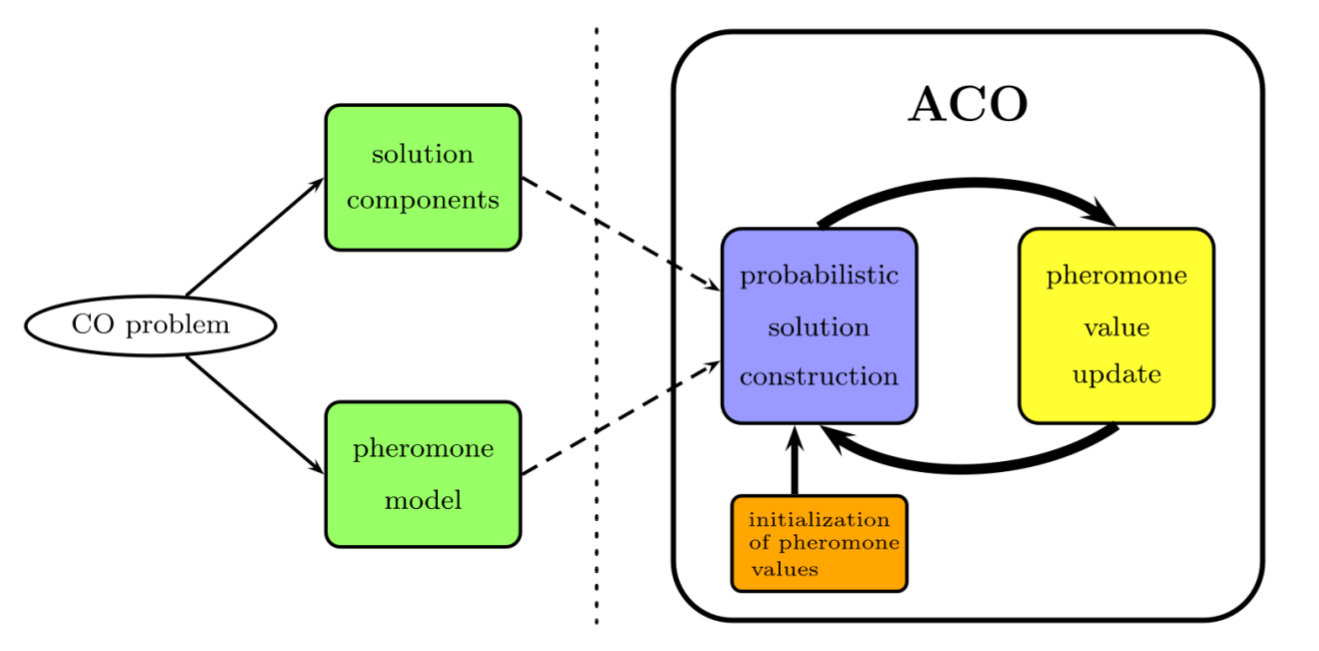
\includegraphics[width=0.8 \linewidth]
      {imgs/meta_heuristica_aco}
      \caption{Diagrama de Funcionamento da Meta-Heurística do ACO}
    \end{figure}
  \end{block}
}

%\frame{
%  \frametitle{Otimização da Colonia de Formigas}
%  \begin{block}{}
%    \begin{figure}[ht]
%      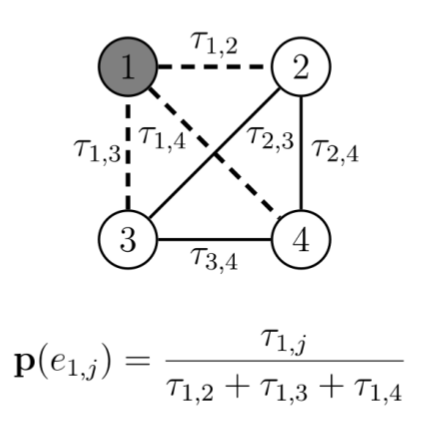
\includegraphics[width=0.4 \linewidth, height = 0.4 \linewidth]{imgs/exemplo_aco_1}
%      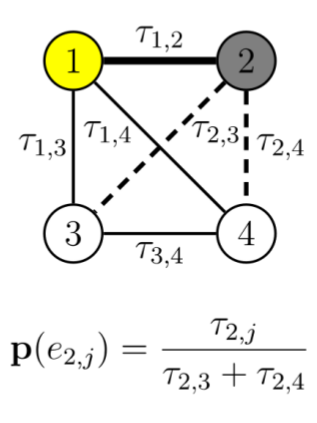
\includegraphics[width=0.3 \linewidth, height = 0.4 \linewidth]{imgs/exemplo_aco_2}
%      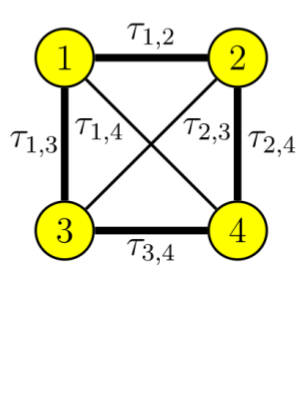
\includegraphics[width=0.3 \linewidth, height = 0.4 \linewidth]{imgs/exemplo_aco_3}
%
%     \caption{Exemplo da construção da solução para o TSP problem}
%    \end{figure}
%  \end{block}
%}

\frame{
  \frametitle{Recozimento Simulado}
  \begin{block}{}
    \begin{figure}
      \centering
      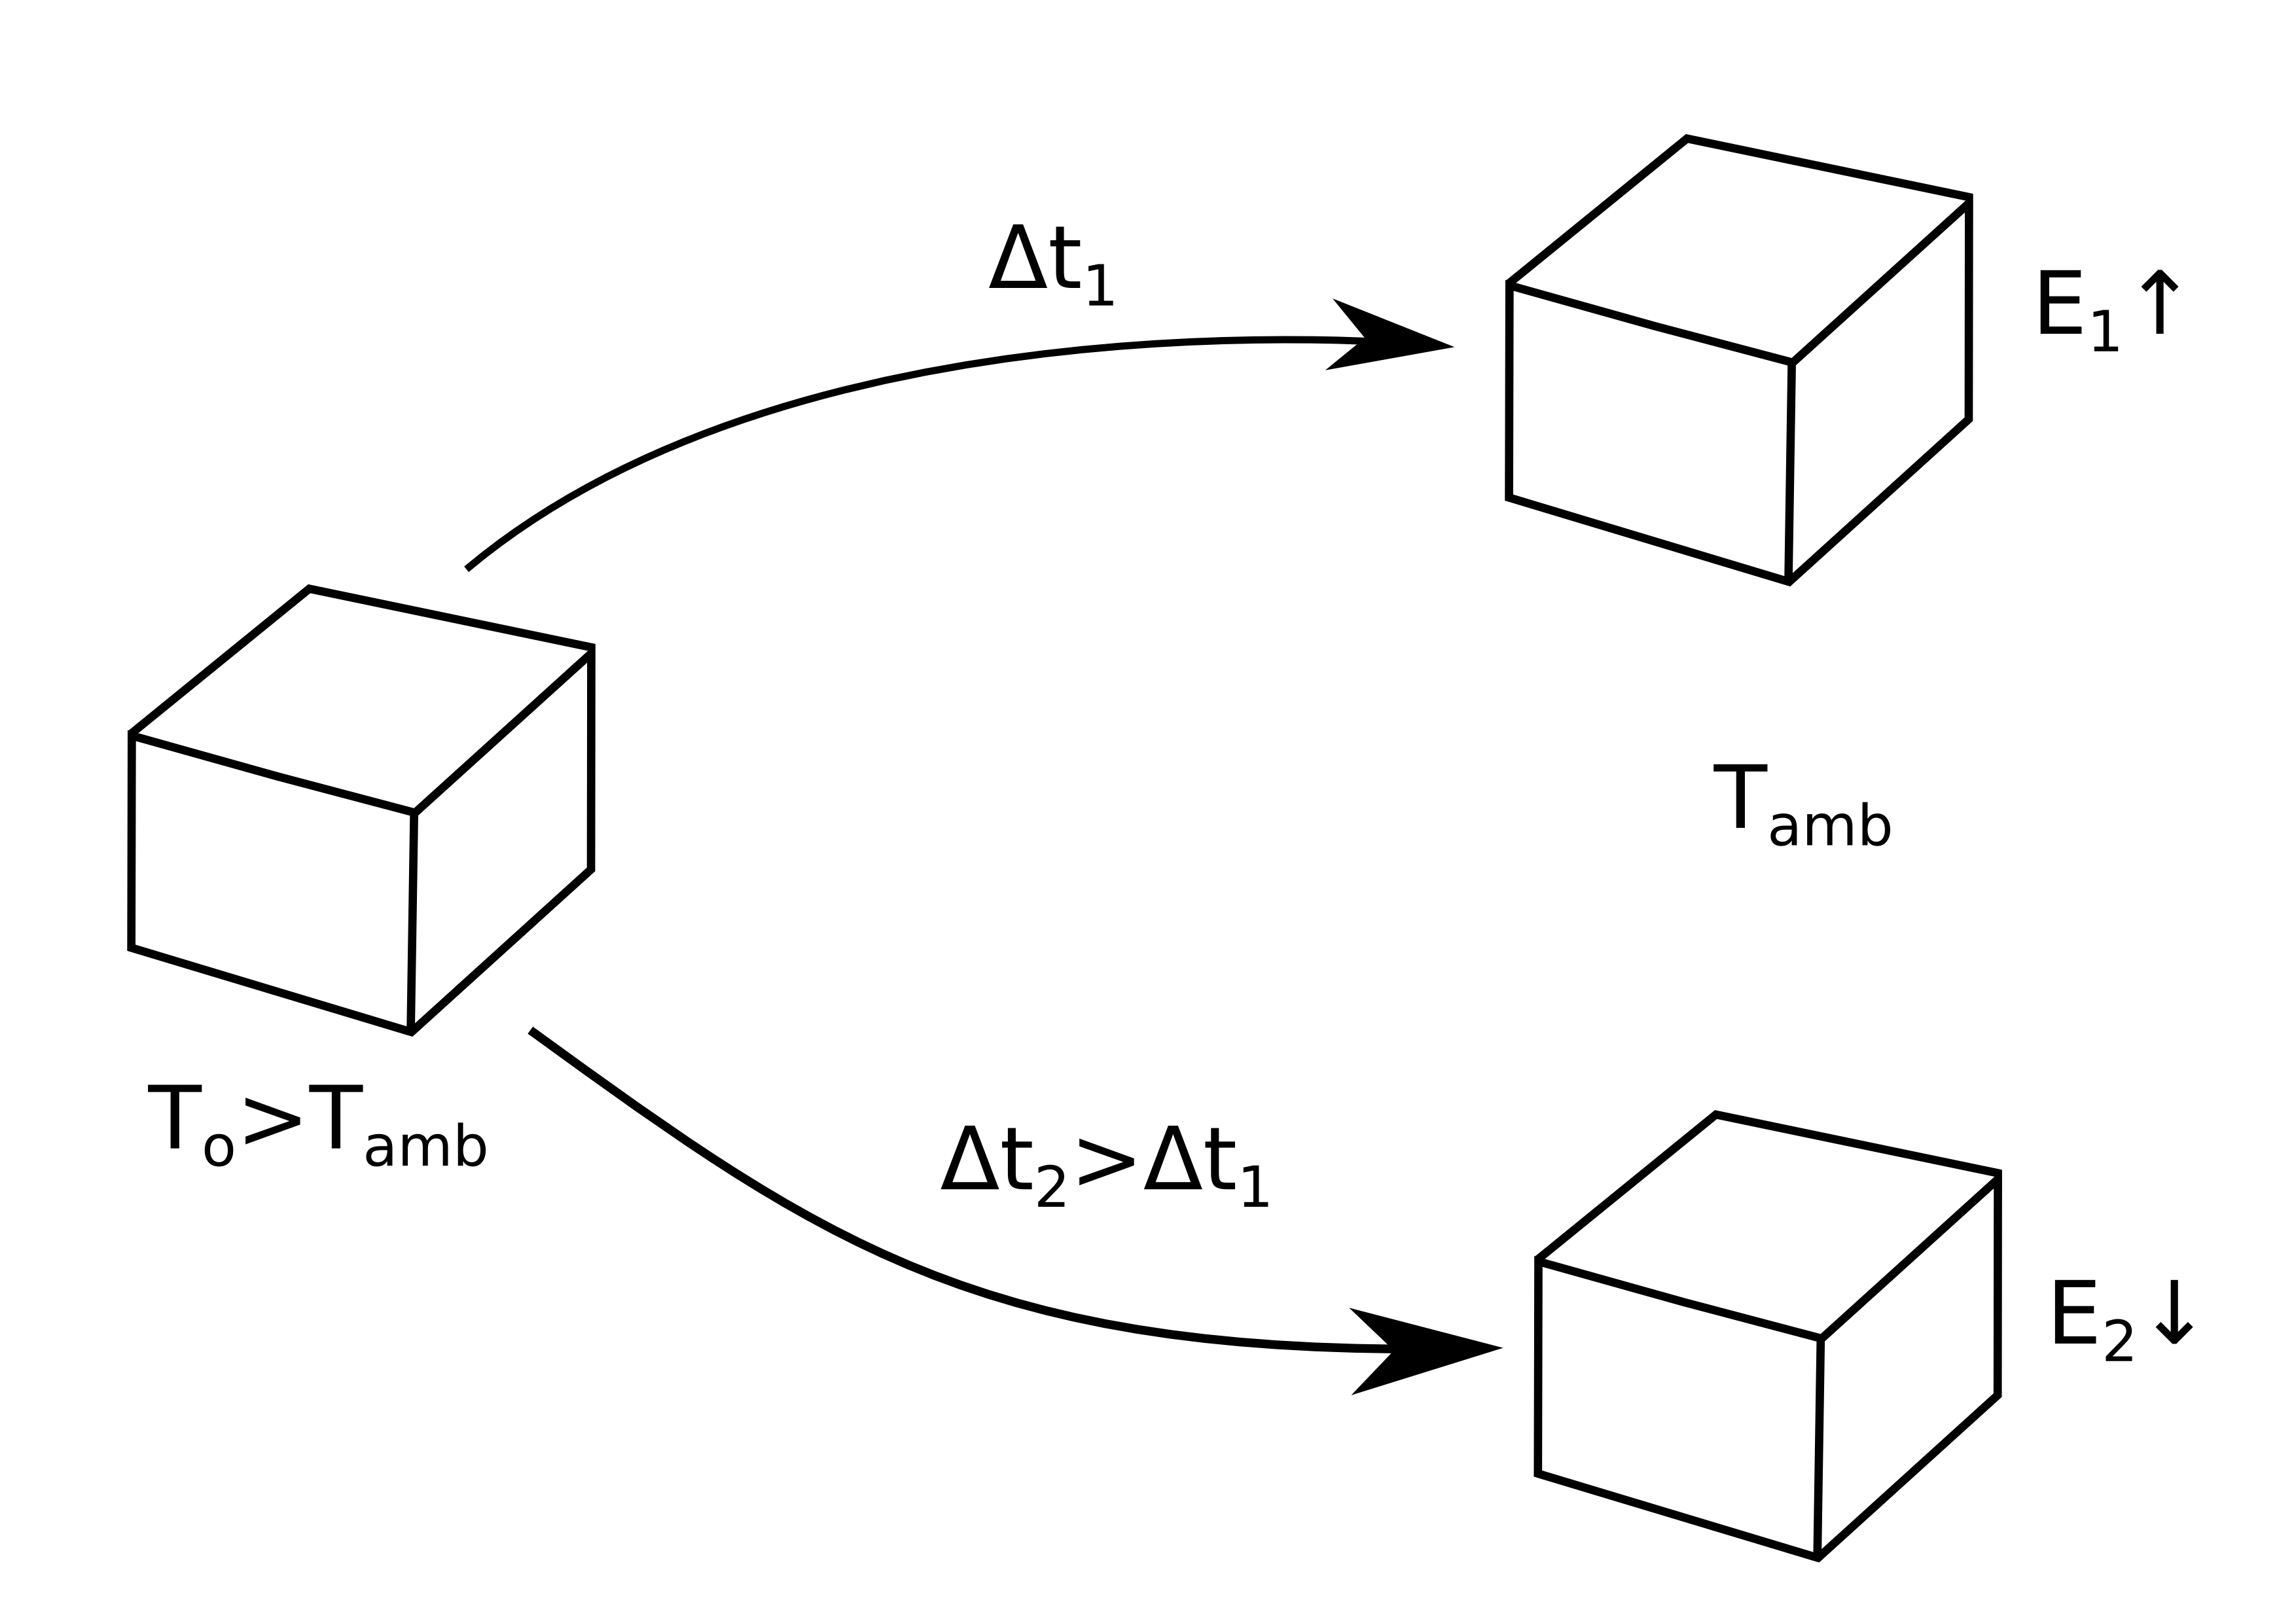
\includegraphics[width = 0.6 \linewidth]{imgs/ilustrativa_sa}
      \caption{Idéia Básica do SA}
    \end{figure}
  \end{block}
}

\frame{
  \frametitle{Recozimento Simulado}
  \begin{block}{}
    \begin{figure}
      \centering
      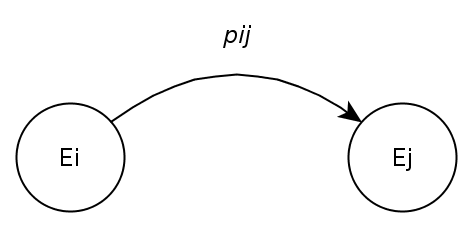
\includegraphics[width = 0.5 \linewidth]{imgs/transicao_sa}
      \caption{Probabilidade da Transição do Estado $i$ para o Estado $j$}
    \end{figure}
  \end{block}
  \begin{block}{}
    $$p_{ij}=\left\{\begin{array}{rc}
    1,&\mbox{se}\quad E\lbrace r_j \rbrace \le E\lbrace r_i \rbrace\\
    e^{\frac{- E\lbrace r_j \rbrace - E\lbrace r_i \rbrace}{k_B T} }, &\mbox{se}\quad 
    E\lbrace r_j \rbrace > E\lbrace r_i \rbrace
    \end{array}\right.
    $$
  \end{block}
}

%\frame{
%  \frametitle{Recozimento Simulado}
%  \begin{block}{}
%    Elementos básicos do SA:
%    \begin{itemize}
%      \item $S$, espaço de estado finito
%      \item $J: S \rightarrow \mathbb{R}$, função de custo
%      \item $S(i) \subset S - \lbrace i \rbrace$ para cada $i \in S$
%      \item $q_{ij}, j \in S(i)$, tal que $\sum_{j \in S_{i}} q_{ij} = 1$
%      \item $T: \mathbb{N} \rightarrow (0, \infty)$, rotina de resfriamento
%      \item $x(0) \in S$, estado inicial
%    \end{itemize}
%  \end{block}
%}
\frame{
\frametitle{Algoritmo Genético}
\begin{block}{}
\subsection{Pseudo código de um Algorítimo Genético}

%\begin{lstlisting}
\begin{algorithm}[H]
\SetKwBlock{Procedimento}{Procedimento}{fim}

%Algorithm: GA(n, \ki, \mu)
\Procedimento{
  %// Initialise generation 0:
  $k \leftarrow 0$, $P_k \leftarrow n$ indivíduos aleatórios\;
  %// EvaluatePk:
  %\Para{cada $i$ em $P_k$}
  %Compute fitness(i) for each i ∈ Pk;
  %Computar a $avaliacao(i)$ para cada $i$ em $P_k$\;
  %while fitness of fittest individual in Pk is not high enough;
  %\Enqto{a $avaliacao(i)$ de cada $i$ em $P_k$ não for boa o suficiente}{
  \Enqto{$avaliacao(i) < desejado$ de cada $i$ em $P_k$}{
    %// Create generation k + 1:
    %// 1. Copy:
    %Select (1−χ)×n members ofPk and insert into Pk+1;
    Selecionar os $(1 - \chi) \times n$ membros com maior $avaliacao(i)$ de $P_k$ e inserir em $P_{k+1}$\;
    %// 2. Crossover:
    %Select χ×n members of Pk; pair them up; produce offspring; insert the offspring into Pk+1;
    Selecionar $\chi \times n$ membros de $P_k$, pareá-los e inserir a cria em $P_{k+1}$\;
    %// 3. Mutate:
    %Select µ×n members of Pk+1; invert a randomly-selected bit in each;
    Selecionar os $\mu \times n$ membros de $P_{k+1}$ com maior $avaliacao(i)$ e inverter um bit aleatório de cada membro\;
    %// Evaluate Pk+1:
    %Compute fitness(i) for each i ∈ Pk;
    %Computar a $avaliacao(i)$ para cada $i$ em $P_{k+1}$\;
    %// Increment:
    %k := k + 1;
    $k \leftarrow k + 1$\;
  }
%return the fittest individual from Pk;ut your code here.
  \Retorna{membro $i$ em $P_k$ com maior $avaliacao(i)$}
}
\caption{Pseudo código de um Algoritmo Genético}
\end{algorithm}
\end{block}
}

\frame{
\frametitle{Redes Neurais}
\begin{block}{}
\begin{figure}[H]
\centering
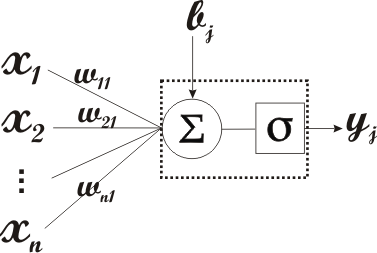
\includegraphics[width=10cm]{figuras/rede_neural_neuronio}
\caption{Modelo matemático de um neurônio.}
\end{figure}
\end{block}
}

\frame{
\frametitle{Redes Neurais}
\begin{block}{}
\begin{figure}[H]
\centering
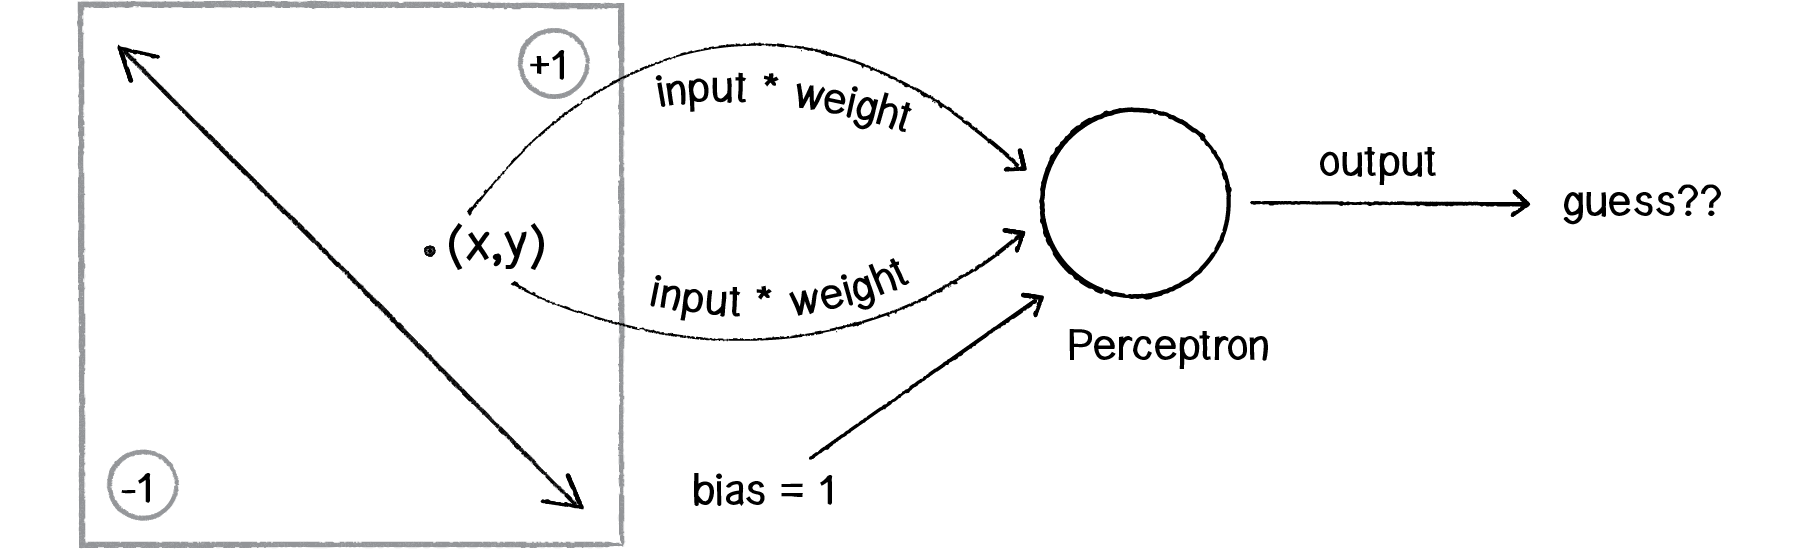
\includegraphics[width=10cm]{figuras/rede_neural_simple_problem}
\caption{\textit{Perceptron} para decidir região de um ponto no plano.}
\end{figure}
\end{block}
}

\frame{
\frametitle{Redes Neurais}
\begin{block}{}
\begin{figure}[H]
\centering
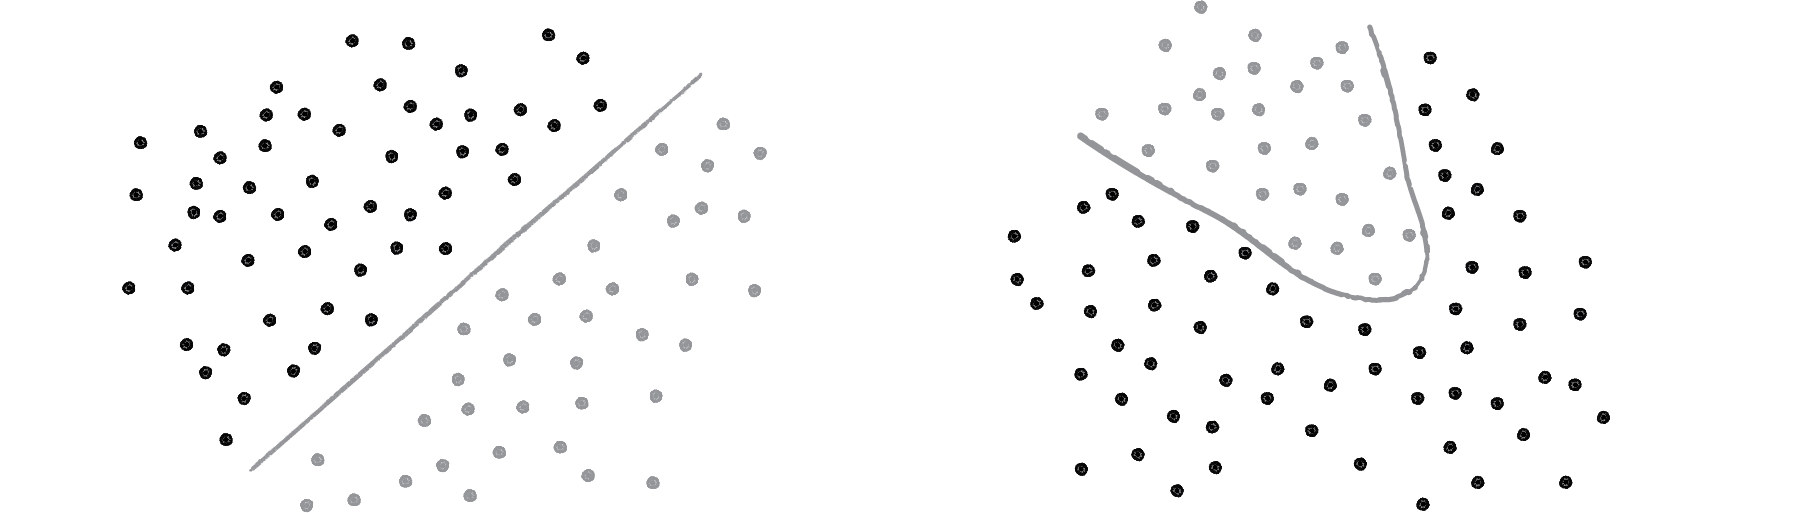
\includegraphics[width=10cm]{figuras/rede_neural_linear_probl}
\caption{Problemas linearmente separáveis vs. não linearmente separáveis.}
\end{figure}
\end{block}
}

\frame{
\frametitle{Redes Neurais}
\begin{block}{}
\begin{figure}[H]
\centering
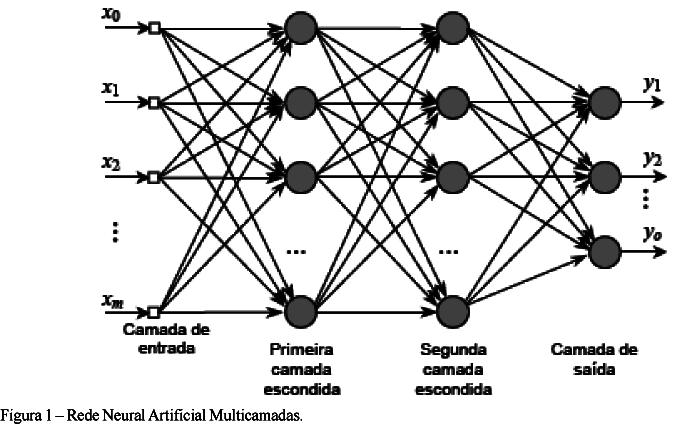
\includegraphics[width=8cm]{figuras/rede_neural_topologia}
\caption{Topoligia de camadas.}
\end{figure}
\end{block}
}
